% !TEX root = ./rep.tex
\section{Demonstration simulation}
\label{s:demo}

To demonstrate the new capability of Cardinal we demonstrate here the use of Cardinal on Summit to perform coupled multi-physics simulations of pebble beds.

\subsection{Numerical Setup}

The case presented here comprises 1568 pebbles. The pebble configuration has been obtained using a discrete element method (DEM) code. A major overhaul on the mesh generation  for the fluid domain has been necessary to automatize as much as possible the process and reduce the number of elements per pebble. The new meshing tool is based on a Voronoi cell strategy. It has allowed to produce high quality hexahedral meshes, while reducing the mesh count to roughly 300-400 elements per pebble.

Examples for these meshes are provided in Figure~\ref{f:ndemo1} for the 1568 pebble configuration and in Figure~\ref{f:ndemo2} for a pebble configuration with over 3,000 pebbles. Both meshes have a similar density.

We note that 1568 pebbles is a significant size for a coupled calculation and representative for instance of the SANA experiments.

\begin{figure}[!h]
\centering
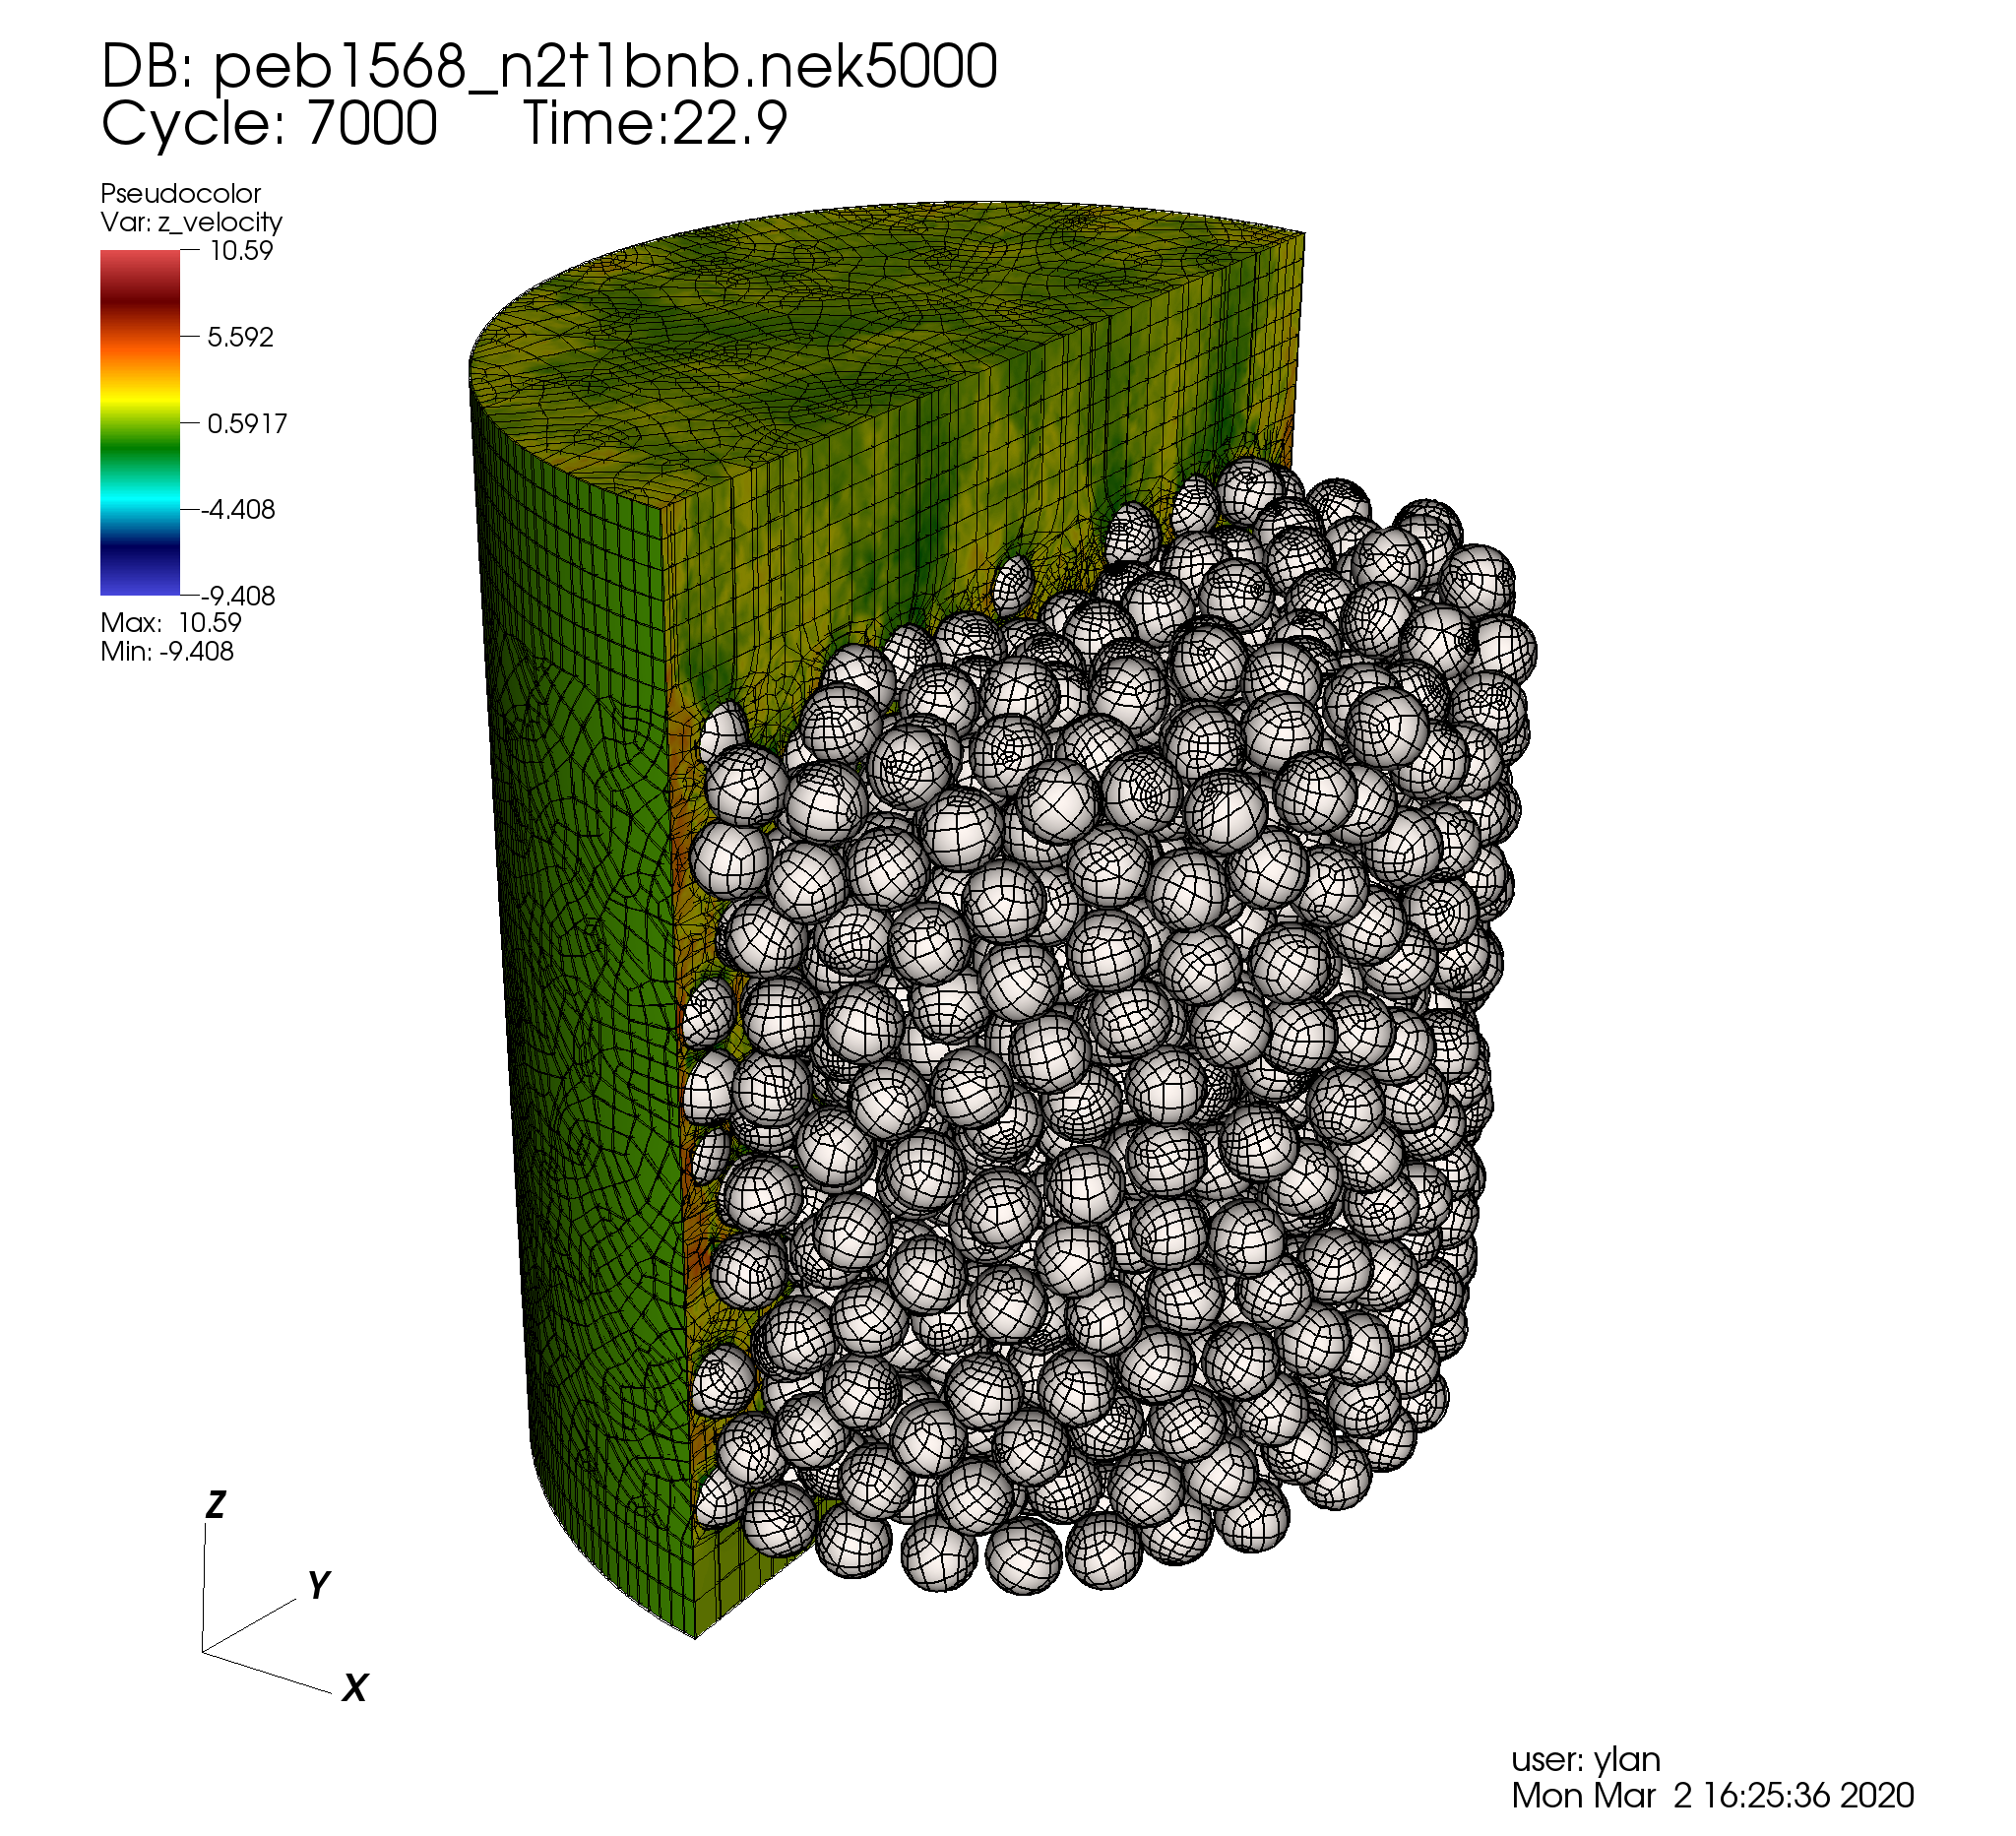
\includegraphics[clip=true,width=0.9\textwidth]{Figures/ndemo_r1}
\caption{NekRS Mesh for 1568 pebble configuration}
\label{f:ndemo1}
\end{figure}

\begin{figure}[!h]
\centering
\includegraphics[clip=true,width=0.9\textwidth]{Figures/ndemo_r2}
\caption{NekRS Mesh for 3260 pebble configuration}
\label{f:ndemo2}
\end{figure}

For this demonstrations, the sizes and composition of the TRISO particles were based on TRISO manufactured
at INL, following the practice established in the previous report \cite{cardinal}. Though these particles were developed for the Advanced Gas Reactor (AGR) fuel, particles with the same specifications are used for FHR test reactors and computations benchmarks. The sizes and compositions of the pebbles were taken from the Mark-1 FHR reactor constructed at UC Berkeley.

For BISON, and the demonstration problem under consideration we consider only the conduction equation and as such it is a relatively straightforward setup. Properties are constant and adapted from available correlations. The mesh for a single sphere is generated and replicated at run time. The same mesh is used for the mesh tallies in OpenMC.

\subsection{Results}

The model described in the previous section has been run on 12 and 20 nodes of Summit, with 6 MPI ranks on each node, corresponding to the 6 GPU on each node. The OpenMC and BISON models are designed to run on CPU while the NekRS model runs on the GPU.

Stand-alone NekRS simulations have been run first up to 25 convective time units to develop turbulence - Figure~\ref{f:ndemo3} using a Large Eddy Simulation (LES) approach.

 A restart file has then been generated and used to restart a transient simulation in Cardinal representing an heat-up of the pebbles. The time step has been fixed to $5*10^-4 s$ in both BISON and NekRS. The temperature at time zero has been set to 300 C everywhere. Figure~\ref{f:ndemo4} presents the temperature at the surface of the pebbles in BISON at three points in time. The simulations took 2.5s per coupled time step on 20 nodes, requiring transfer between physics at each time step. However this could be greatly optimized by relaxing the requirement, as data transfer from GPU to CPU should be minimized as much as possible.

\begin{figure}[!h]
\centering
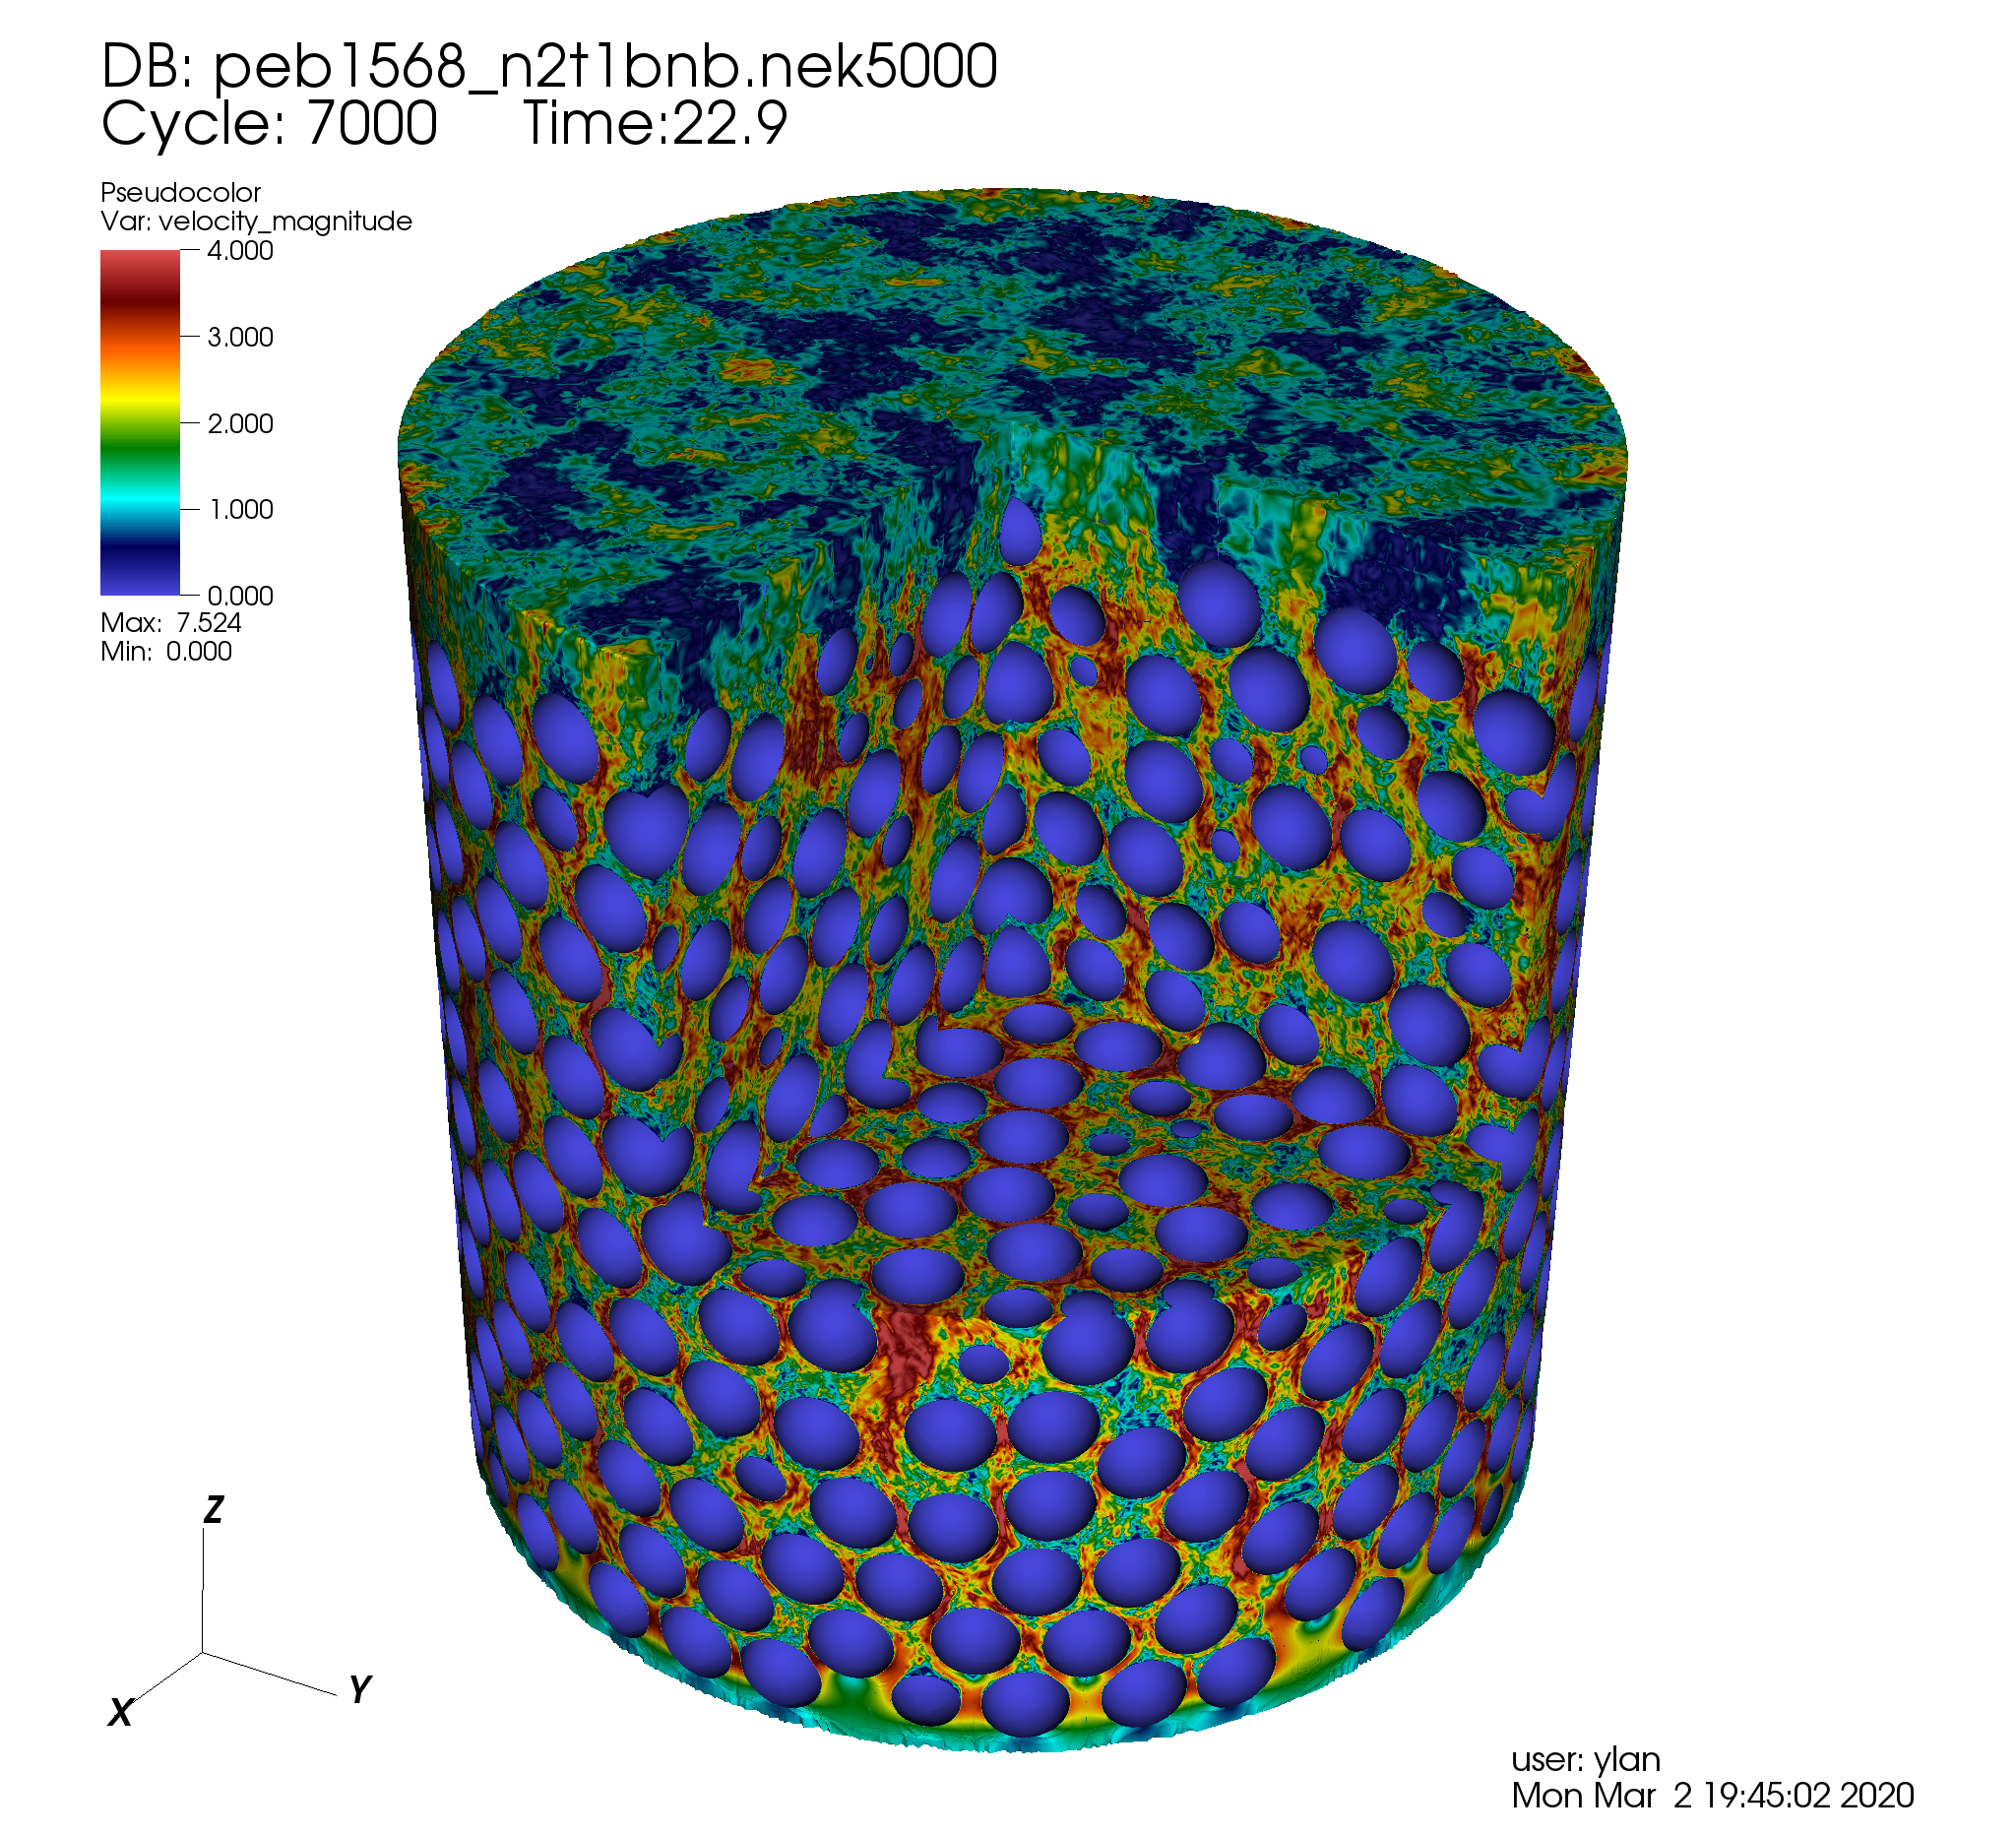
\includegraphics[clip=true,width=0.9\textwidth]{Figures/ndemo_r3}
\caption{NekRS results for the velocity field.}
\label{f:ndemo3}
\end{figure}


\begin{figure}[!h]
\centering
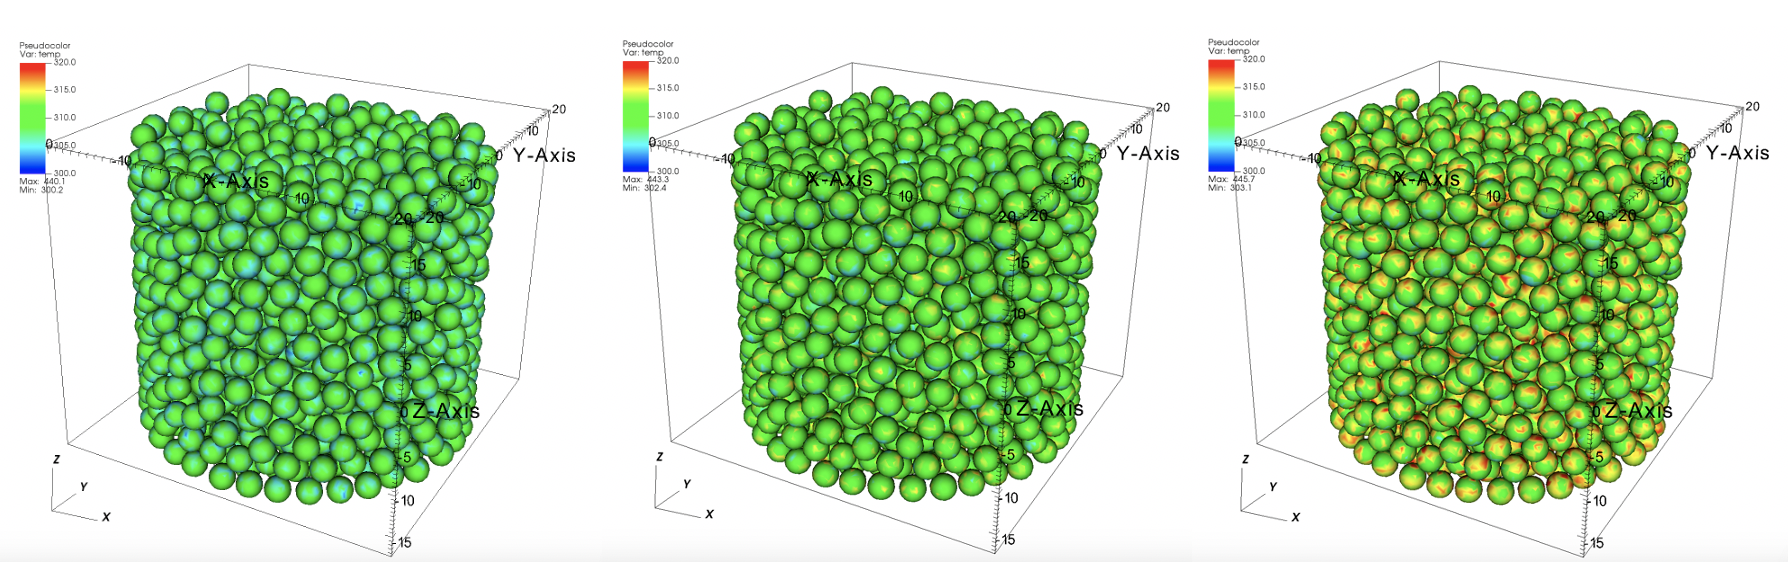
\includegraphics[clip=true,width=0.9\textwidth]{Figures/ndemo_r4}
\caption{Temperature result for the pebble surface temperature at three points in time.}
\label{f:ndemo4}
\end{figure}

The results of OpenMC simulations coupled with the heat conduction module are shown in Figures ~\ref{f:1568_openmc_heat_source} and ~\ref{f:1568_openmc_temperatures} with the same time step parameters as in the NekRS simulations described above. An eigenvalue simulation using 50,000 particles in 150 batches with 50 inactive batches was performed in each time step. While the eigenvalue in this simulation is well-converged (to within 20 pcm), the unstructured mesh heat source contains more noise than the pebble-averaged heat source due to the smaller number of samples per bin in the tally. Production simulations may require a higher number of particles per batch to more tightly converge the heating distribution when using the unstructured mesh tally source. Figure~\ref{f:1568_openmc_temperatures_single_pebble} demonstrates the effect of the improved spatial resolution provided by the unstructured mesh heat source from OpenMC on the temperature distribution within a representative pebble. In the case of the pebble-averaged heat source the temperature profile is nearly perfectly symmetric, reflecting the uniform heat source applied in that region, while an asymmetry can be seen in the profile generated from the unstructured mesh heat source indicating that the distribution of this source has an impact on the temperature distribution in the solid and resulting heat transfer to the fluid.

\begin{figure}[!h]
\centering
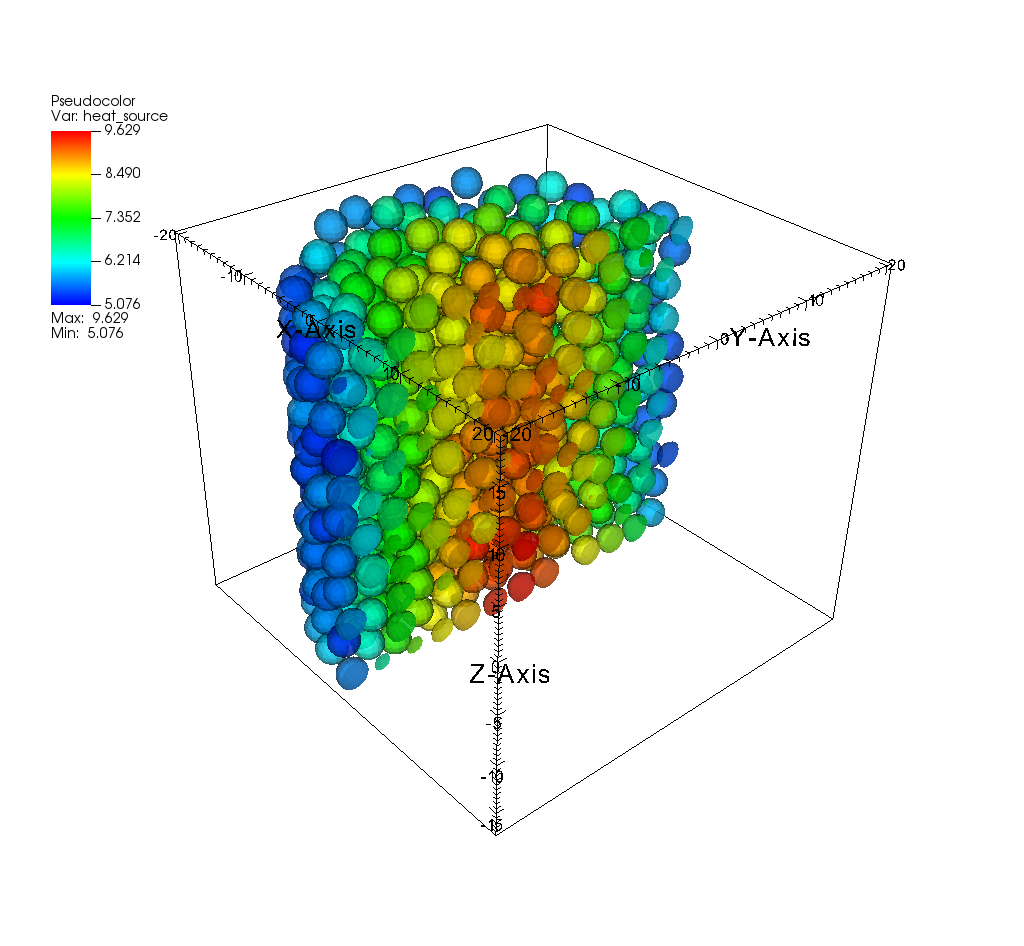
\includegraphics[clip=true,width=0.48\textwidth]{Figures/openmc_cell_heat_source}
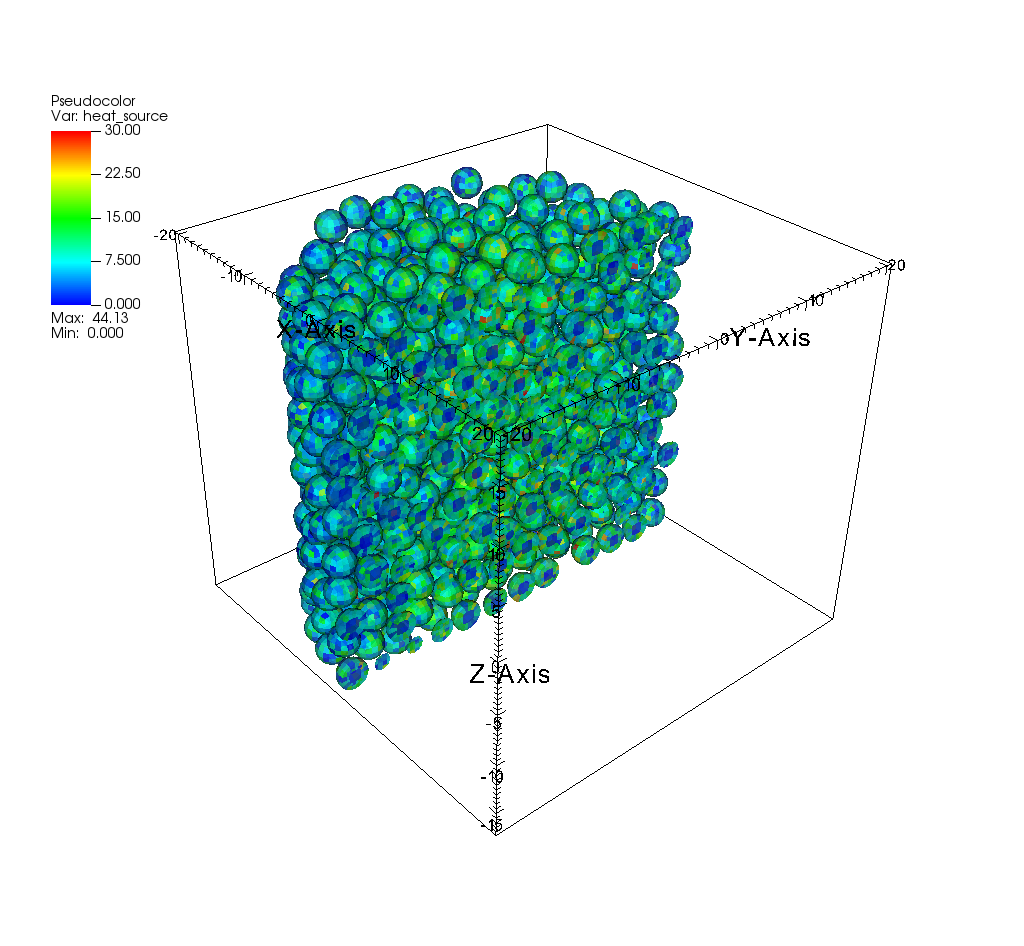
\includegraphics[clip=true,width=0.48\textwidth]{Figures/openmc_mesh_heat_source}
\caption{Left: Heat source using the original cell tallies to produces an average heat source per-pebble. Right: Heat source produced using an OpenMC unstructured mesh tally.}
\label{f:1568_openmc_heat_source}
\end{figure}

\begin{figure}[!h]
\centering
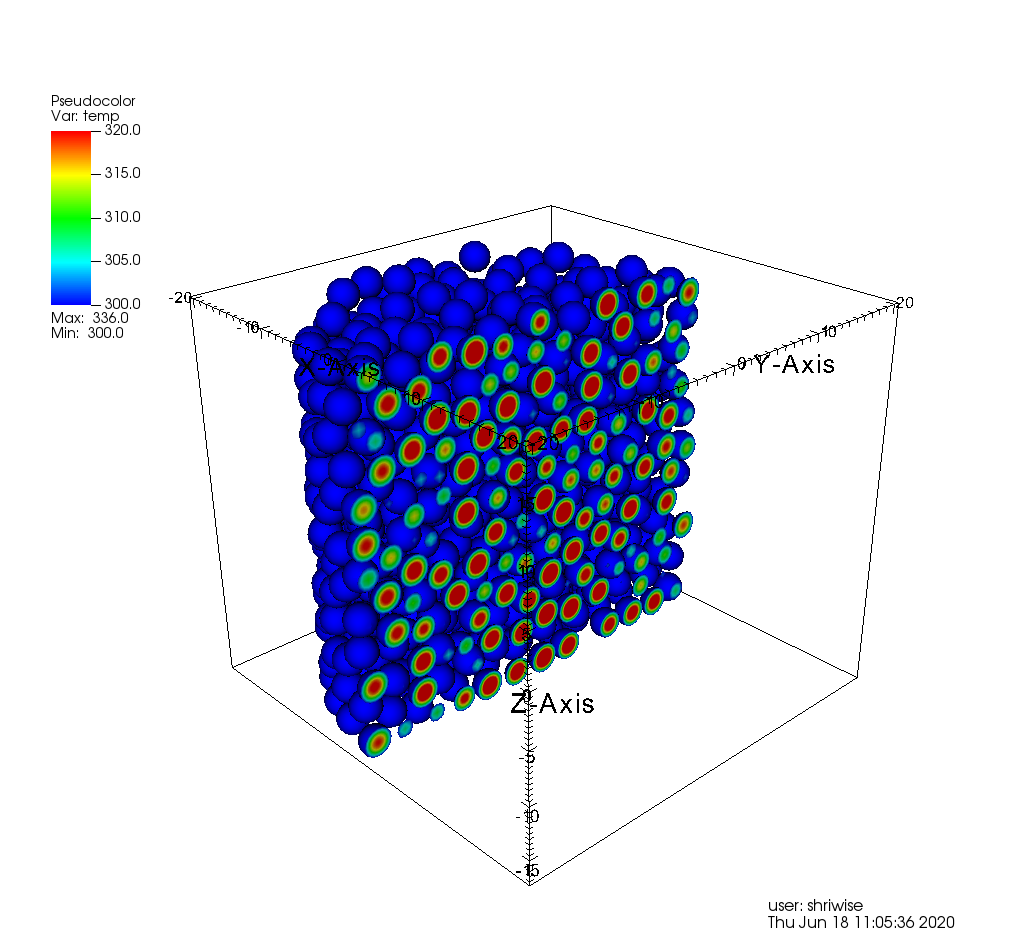
\includegraphics[clip=true,width=0.48\textwidth]{Figures/openmc_cell_temperature}
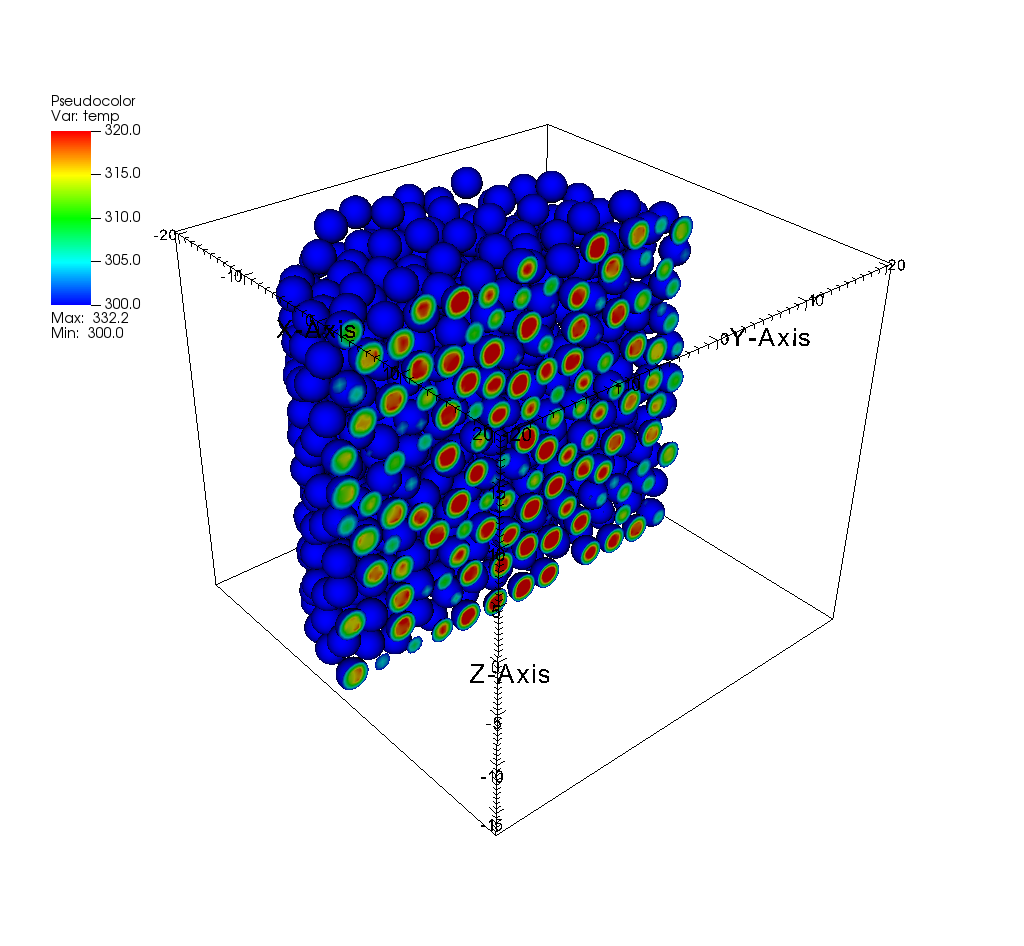
\includegraphics[clip=true,width=0.48\textwidth]{Figures/openmc_mesh_temperature}
\caption{Left: Temperature in the solid resulting from the cell-based heating tally. Right: Temperature in the solid resulting from the unstructured mesh heating tally in OpenMC.}
\label{f:1568_openmc_temperatures}
\end{figure}

\begin{figure}[!h]
\centering
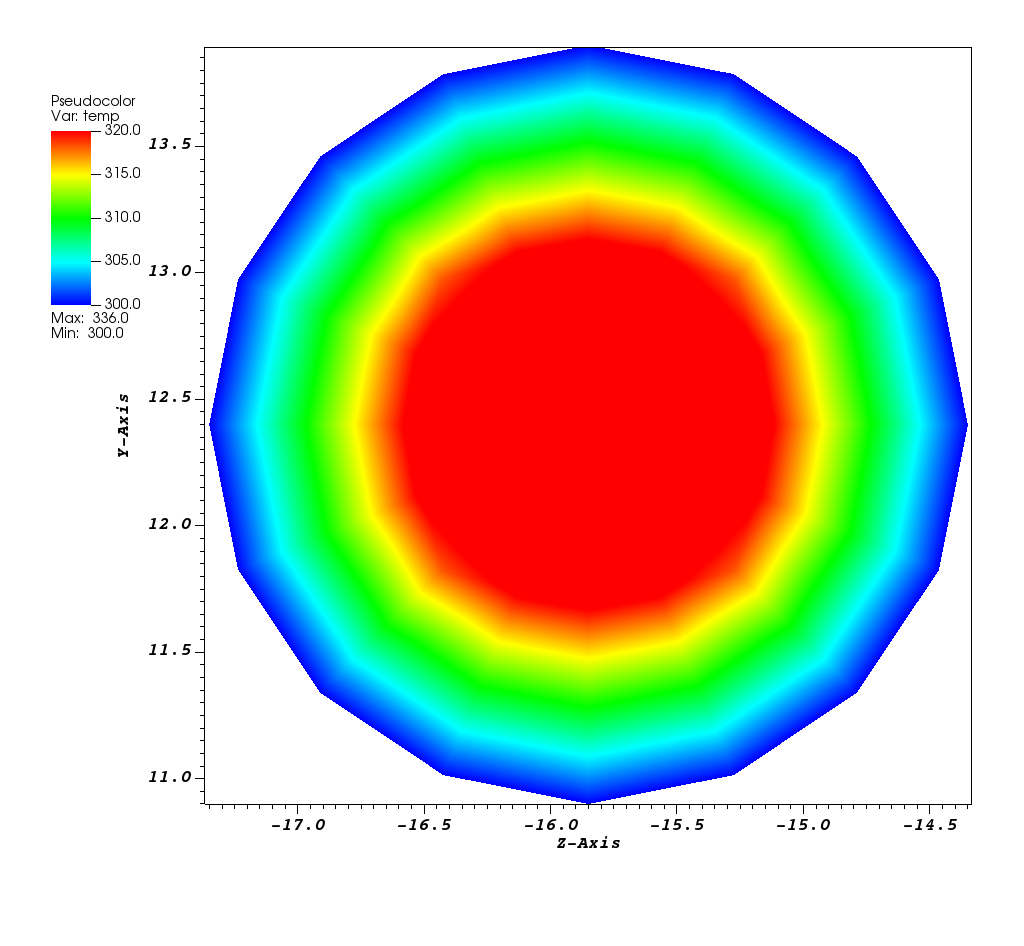
\includegraphics[clip=true,width=0.48\textwidth]{Figures/openmc_cell_temperature_zoomed}
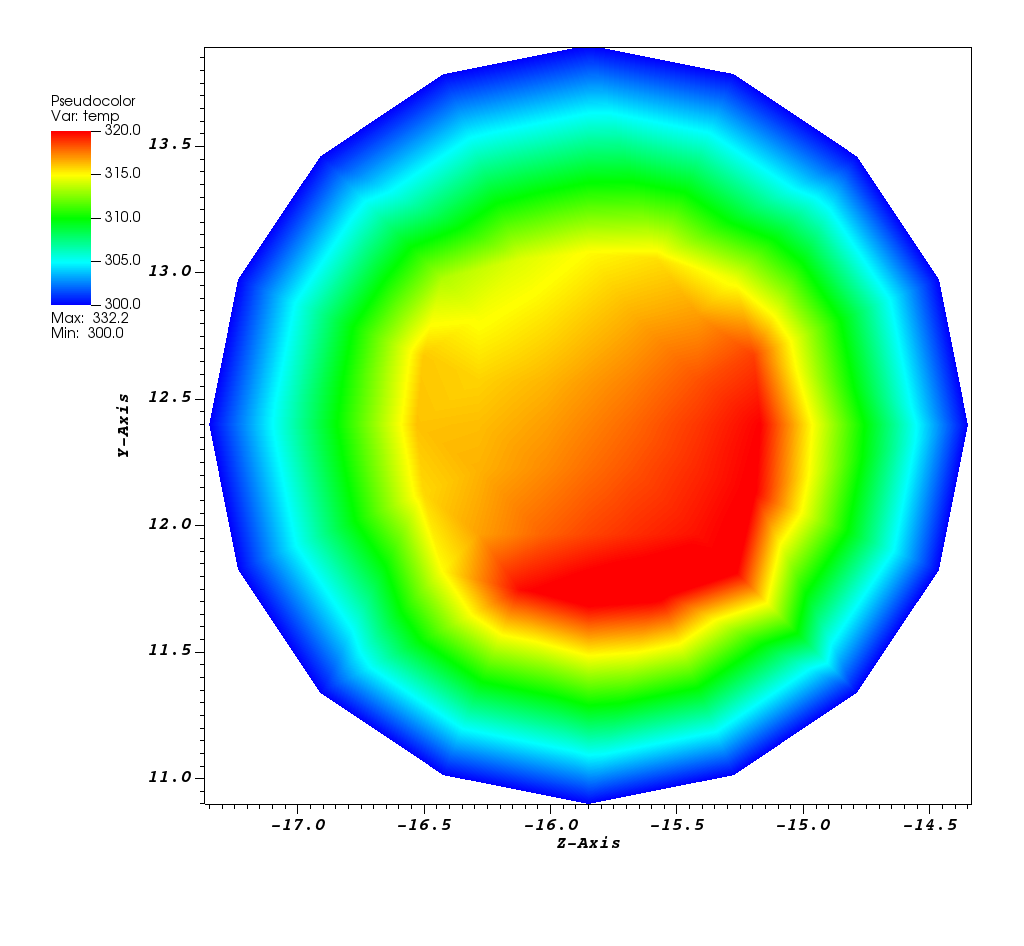
\includegraphics[clip=true,width=0.48\textwidth]{Figures/openmc_mesh_temperature_zoomed}
\caption{Temperature profiles of the same pebble in the 1568 pebble demo using the pebble-averaged heating (left) and the unstructured mesh heating (right).}
\label{f:1568_openmc_temperatures_single_pebble}
\end{figure}

\subsection{Projection to full core}

20 nodes of Summit represents less than 1\% of the computing power available on Summit. We estimate that 80\% of the machine will be sufficient to perform full core calculation in FHRs corresponding to 300,000 pebbles.
